% LaTeX source for ``Think DSP: Digital Signal Processing for Programmers''
% Copyright 2013  Allen B. Downey.

% License: Creative Commons Attribution-NonCommercial 3.0 Unported License.
% http://creativecommons.org/licenses/by-nc/3.0/
%

\documentclass[12pt]{book}
\usepackage[width=5.5in,height=8.5in,
  hmarginratio=3:2,vmarginratio=1:1]{geometry}

% for some of these packages, you might have to install
% texlive-latex-extra (in Ubuntu)

\usepackage[T1]{fontenc}
\usepackage{textcomp}
\usepackage{mathpazo}
\usepackage{url}
\usepackage{graphicx}
\usepackage{subfig}
\usepackage{amsmath}
\usepackage{amsthm}
\usepackage{makeidx}
\usepackage{setspace}
\usepackage{hevea}                           
\usepackage{upquote}
\usepackage{fancyhdr}
\usepackage[bookmarks]{hyperref}

\title{Think DSP}
\author{Allen B. Downey}

\newcommand{\thetitle}{Think DSP: Digital Signal Processing in Python}
\newcommand{\theversion}{0.2}

% these styles get translated in CSS for the HTML version
\newstyle{a:link}{color:black;}
\newstyle{p+p}{margin-top:1em;margin-bottom:1em}
\newstyle{img}{border:0px}

% change the arrows in the HTML version
\setlinkstext
  {\imgsrc[ALT="Previous"]{back.png}}
  {\imgsrc[ALT="Up"]{up.png}}
  {\imgsrc[ALT="Next"]{next.png}} 

\makeindex

\newif\ifplastex
\plastexfalse

\begin{document}

\frontmatter

\ifplastex

\else
\fi

\ifplastex
    \usepackage{localdef}
    \maketitle

\else

\newtheoremstyle{exercise}% name of the style to be used
  {\topsep}% measure of space to leave above the theorem. E.g.: 3pt
  {\topsep}% measure of space to leave below the theorem. E.g.: 3pt
  {}% name of font to use in the body of the theorem
  {0pt}% measure of space to indent
  {\bfseries}% name of head font
  {}% punctuation between head and body
  { }% space after theorem head; " " = normal interword space
  {}% Manually specify head

\theoremstyle{exercise}
\newtheorem{exercise}{Exercise}[chapter]

\input{latexonly}

\begin{latexonly}

\renewcommand{\blankpage}{\thispagestyle{empty} \quad \newpage}

% TITLE PAGES FOR LATEX VERSION

%-half title--------------------------------------------------
\thispagestyle{empty}

\begin{flushright}
\vspace*{2.0in}

\begin{spacing}{3}
{\huge Think DSP}\\
{\Large Digital Signal Processing in Python}
\end{spacing}

\vspace{0.25in}

Version \theversion

\vfill

\end{flushright}

%--verso------------------------------------------------------

\blankpage
\blankpage

%--title page--------------------------------------------------
\pagebreak
\thispagestyle{empty}

\begin{flushright}
\vspace*{2.0in}

\begin{spacing}{3}
{\huge Think DSP}\\
{\Large Digital Signal Processing in Python}
\end{spacing}

\vspace{0.25in}

Version \theversion

\vspace{1in}


{\Large
Allen B. Downey\\
}


\vspace{0.5in}

{\Large Green Tea Press}

{\small Needham, Massachusetts}

\vfill

\end{flushright}


%--copyright--------------------------------------------------
\pagebreak
\thispagestyle{empty}

Copyright \copyright ~2013 Allen B. Downey.


\vspace{0.2in}

\begin{flushleft}
Green Tea Press       \\
9 Washburn Ave \\
Needham MA 02492
\end{flushleft}

Permission is granted to copy, distribute, and/or modify this document
under the terms of the Creative Commons Attribution-NonCommercial 3.0 Unported
License, which is available at \url{http://creativecommons.org/licenses/by-nc/3.0/}.

\vspace{0.2in}

\end{latexonly}


% HTMLONLY

\begin{htmlonly}

% TITLE PAGE FOR HTML VERSION

{\Large \thetitle}

{\large Allen B. Downey}

Version \theversion

\vspace{0.25in}

Copyright 2012 Allen B. Downey

\vspace{0.25in}

Permission is granted to copy, distribute, and/or modify this document
under the terms of the Creative Commons Attribution-NonCommercial 3.0
Unported License, which is available at
\url{http://creativecommons.org/licenses/by-nc/3.0/}.

\setcounter{chapter}{-1}

\end{htmlonly}

\fi
% END OF THE PART WE SKIP FOR PLASTEX

\chapter{Preface}
\label{preface}

The premise of this book (and the other books in the {\it Think X}
series) is that if you know how to program, you can use that skill to
learn other things.  I am writing this book because I think the
conventional approach to digital signal processing is backward: most
books (and the classes that use them) present the material bottom-up,
starting with mathematical abstractions like phasors.

With a programming-based approach, I can go top-down, which means I
can present the most important ideas right away.  By the end of the
first chapter, you can break down a sound into its harmonics, modify
the harmonics, and generate new sounds.

This is a work in progress, so comments are welcome.


Allen B. Downey \\*

Needham MA \\*

Allen B. Downey is a Professor of Computer Science at 
the Franklin W. Olin College of Engineering.



\section*{Contributor List}

If you have a suggestion or correction, please send email to 
{\tt downey@allendowney.com}.  If I make a change based on your
feedback, I will add you to the contributor list
(unless you ask to be omitted).
\index{contributors}

If you include at least part of the sentence the
error appears in, that makes it easy for me to search.  Page and
section numbers are fine, too, but not as easy to work with.
Thanks!

\small

\begin{itemize}

\item 

% ENDCONTRIB

\end{itemize}

\normalsize

\clearemptydoublepage

% TABLE OF CONTENTS
\begin{latexonly}

\tableofcontents

\clearemptydoublepage

\end{latexonly}

% START THE BOOK
\mainmatter


\chapter{Sounds and signals}
\label{sounds}

A {\bf signal} is a representation of a quantity that varies in time,
or space, or both.  That definition is pretty abstract, so let's start
with a concrete example, sound.  Sound is variation in air pressure.
A sound signal represents variations in air pressure over time.

A microphone is a device that measures these variations and generates
an electronic signal that represents sound.  A speaker is a device
that takes an electrical signal and produces sound.
Microphones and speakers are called {\bf transducers} because they
transduce, or convert, signals from one form to another.

This book is about signal processing, which includes processes for
synthesizing, transforming, and analyzing signals.  It focuses on
sound signals, but the same methods apply to other signals, like
electronic signals and mechanical vibration.

They also apply to signals that vary in space rather than time, like
elevation along a hiking trail.  And they apply to signals in more
than one dimension, like an image, which you can think of as a signal
that varies in two-dimensional space.  Or a movie, which is
a signal that varies in two-dimensional space {\it and} time.

But we start with simple one-dimensional sound.


\section{Periodic signals}

\begin{figure}
% violin.py
\centerline{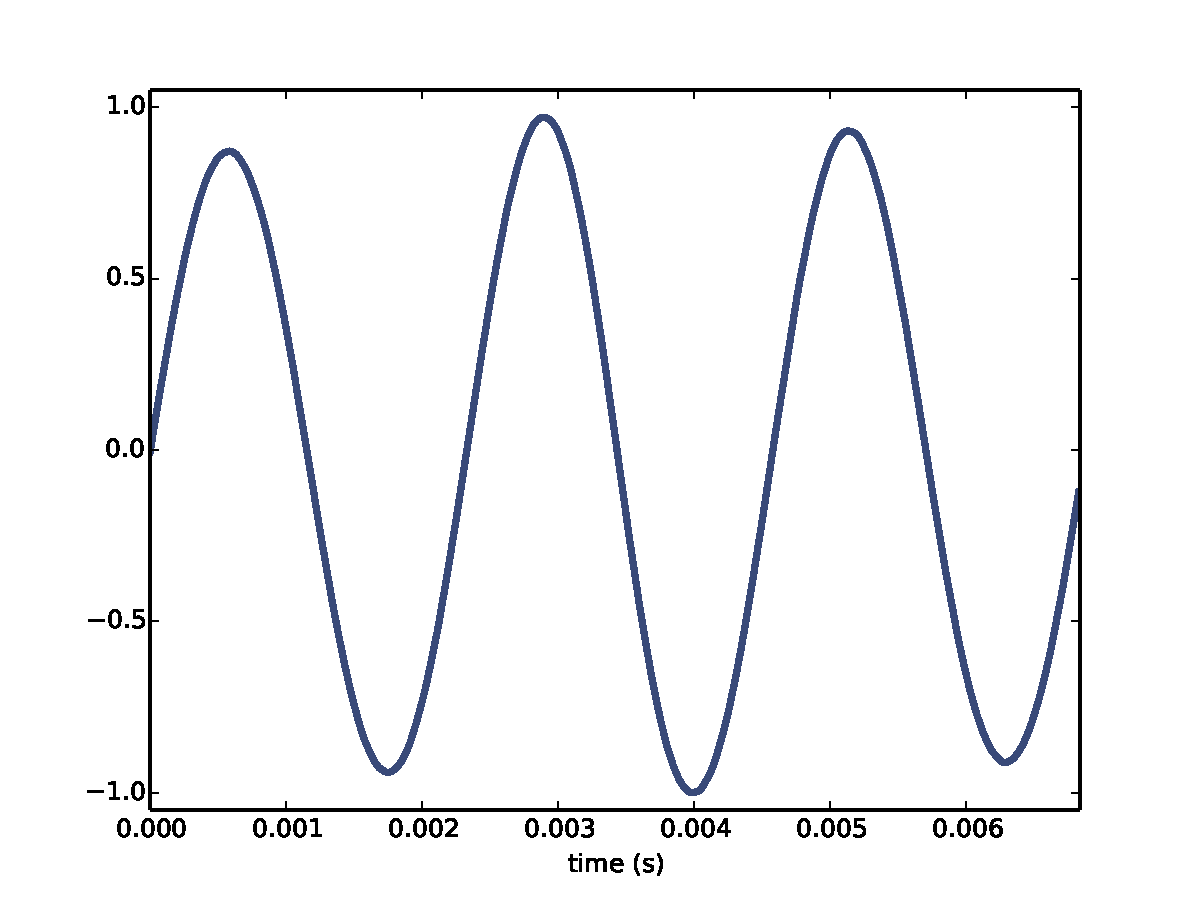
\includegraphics[height=2.5in]{figs/tuning1.pdf}}
\caption{Segment from a recording of a tuning fork.}
\label{fig.tuning1}
\end{figure}

We'll also start with {\bf periodic signals}, which are signals that
repeat themselves after some period of time.  For example, if you
strike a tuning fork, it vibrates and generates sound.  If you record
that sound and plot the transduced signal, it looks like
Figure~\ref{fig.tuning1}.\footnote{I got this recording from
  \url{http://www.freesound.org/people/zippi1/sounds/18871/}.}

This signal is a sinusoid, which means it has the same shape as
the trigonometric sine function. 

You can see that this signal is periodic.  I chose the duration
to show three full periods, also known as {\bf cycles}.
The duration of each cycle is
about 2.3 ms.

The {\bf frequency} of a signal is the number of cycles
per second, which is the inverse of the period.
The units of frequency are cycles per second, or {\bf Hertz},
abbreviated ``Hz''.

The frequency of this signal is about 439 Hz, slightly lower than 440
Hz, which is the standard tuning pitch for orchestral music.  The
musical name of this note is A, or more specifically, A4.  If you are
not familiar with ``scientific pitch notation'', the suffix indicates
which octave the note is in.  A4 is the A above middle C.  A5 is one
octave higher.  See
\url{http://en.wikipedia.org/wiki/Scientific_pitch_notation}.

\begin{figure}
% violin.py
\centerline{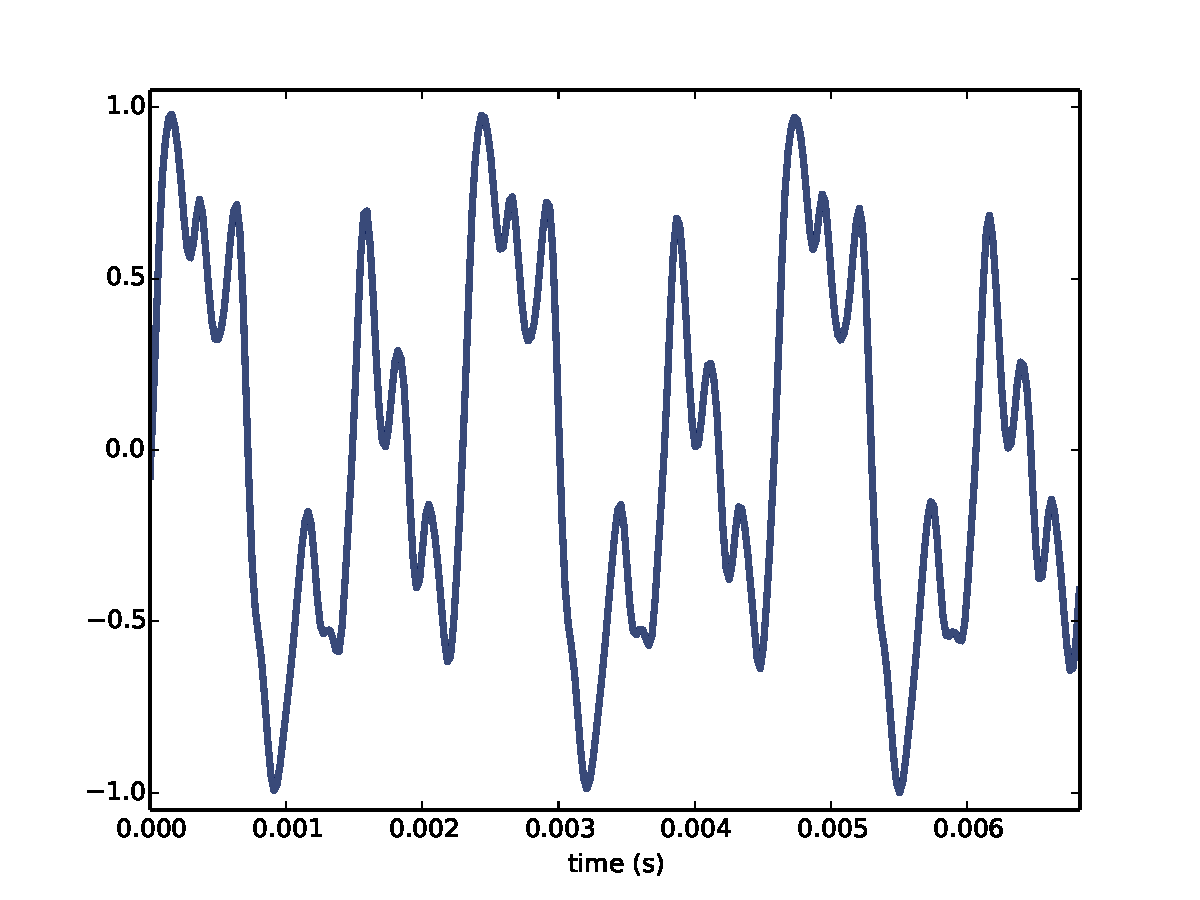
\includegraphics[height=2.5in]{figs/violin1.pdf}}
\caption{Segment from a recording of a violin.}
\label{fig.violin1}
\end{figure}

A tuning fork generates a sinusoid because the vibration of the tines
is a form of simple harmonic motion.  Most musical instruments
produce periodic signals, but the shape of these signals is not
sinusoidal.  For example, Figure~\ref{fig.violin1} shows a segment
from a recording of a violin playing
Boccherini's String Quintet No. 5 in E, 3rd
movement.\footnote{The recording is from
  \url{http://www.freesound.org/people/jcveliz/sounds/92002/}.
I identified the piece using \url{http://www.musipedia.org}.}

% Parson's code: DUUDDUURDR

Again we can see that the signal is periodic, but the shape of the
signal is much more complex.  The shape of a periodic signal is called
the {\bf waveform}.  Most musical instruments produce waveforms more
complex than a sinusoid.  The shape of the waveform determines the
musical {\bf timbre}, which is our perception of the tone quality of the
sound.  People usually perceive complex waveforms as rich, warm and
more interesting than sinusoids.


\section{Spectral decomposition}

\begin{figure}
% violin.py
\centerline{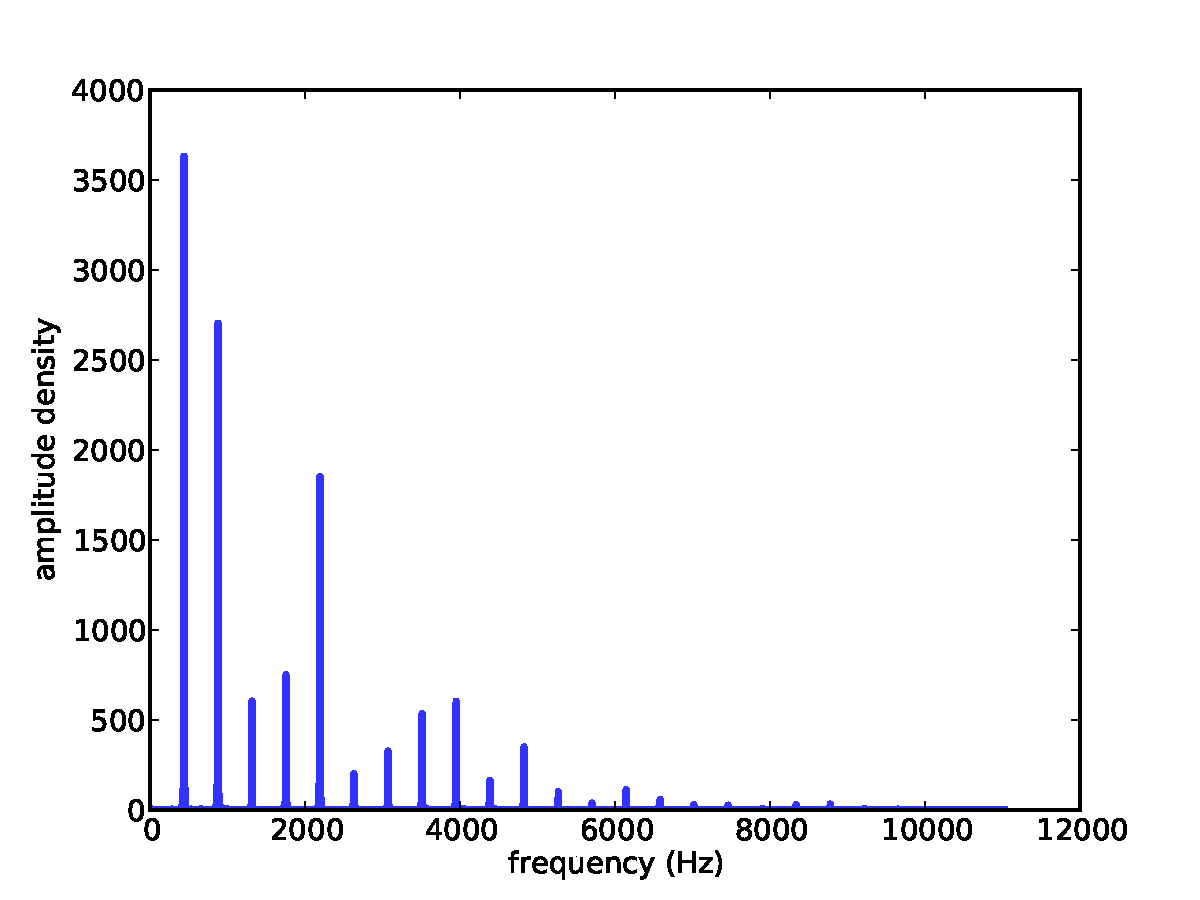
\includegraphics[height=2.5in]{figs/violin2.pdf}}
\caption{Spectrum of a segment from the violin recording.}
\label{fig.violin2}
\end{figure}

The most important idea in this book is {\bf spectral decomposition},
which is the idea that a complex signal can be expressed as the sum of
simpler signals with different frequencies.

And the most important algorithm in this book is the {\bf discrete
  Fourier transform}, or {\bf DFT}, which takes a signal (a quantity
varying in time) and produces its {\bf spectrum}, which is the set of
sinusoids that add up to produce the signal.

For example, Figure~\ref{fig.violin2} shows the spectrum of the violin
recording in Figure~\ref{fig.violin1}.  The x-axis is the range of
frequencies that make up the signal.  The y-axis shows the strength of
each frequency component.

The lowest frequency component is called the {\bf fundamental
  frequency}.  The fundamental frequency of this signal is near 440 Hz
(actually a little lower, or ``flat'').

In this signal the fundamental frequency has the largest amplitude,
so it is also the {\bf dominant frequency}.

Normally the perceived pitch of a sound is determined by the
fundamental frequency, even if it is not dominant. 

The other spikes in the spectrum are at frequencies 880, 1320, 1760, and
2200, which are integer multiples of the fundamental.
These components are called {\bf harmonics} because they are
musically harmonious with the fundamental:

\begin{itemize}

\item 880 is the frequency of
A5, one octave higher than the fundamental.  

\item 1320 is approximately E6, which is a major fifth above A5.

\item 1760 is A6, two octaves above the fundamental. 

\item 2200 is approximately C$\sharp$7, which is a major third
above A6.

\end{itemize}

In other words, these harmonics make up the notes of an A major
chord, although not all in the same octave.  Some of them are only
approximate because the notes that make up Western music have been
adjusted for {\bf equal temperament} (see
 \url{http://en.wikipedia.org/wiki/Equal_temperament}).

Given the harmonics and their amplitudes, you can reconstruct the
signal (at least approximately) by adding up sinusoids.  Or, to
reconstruct the signal exactly, you can use the inverse DFT.  
Next we'll see how.


\section{Signals}

I wrote a Python module called {\tt thinkdsp} that contains
classes and function for working with signals and spectrums.
\footnote{In Latin the plural of ``spectrum'' is ``spectra'', but I
prefer to use standard English plurals.}  You can download
it from \url{http://think-dsp.com/thinkdsp.py}.

To represent signals, {\tt thinkdsp} provides a class named
{\tt Signal}, which is the parent class for several signal types,
including {\tt Sinusoid}, which represents both sine and cosine
signals.

{\tt thinkdsp} provides functions to create sine and cosine signals:

\begin{verbatim}
    cos_sig = thinkdsp.CosSignal(freq=440, amp=1.0, offset=0)
    sin_sig = thinkdsp.SinSignal(freq=880, amp=0.5, offset=0)
\end{verbatim}

{\tt freq} is frequency in Hz.  {\tt amp} is amplitude in arbitrary
units.  {\tt offset} is a {\tt phase offset} in radians.

The phase offset determines where in the period the signal starts
(that is, when {\tt t=0}).  For example, a cosine signal with {\tt
  offset=0} starts at $\cos 0$, which is 1.  With {\tt offset=pi/2} it
starts at $\cos \pi/2$, which is 0.
A sine signal with
{\tt offset=0} also starts at 0.  In fact,
a cosine signal with {\tt offset=pi/2} is identical to a sine
signal with {\tt offset=0}.

Signals have an \verb"__add__" method, so you can use the {\tt +}
operator to add them:

\begin{verbatim}
    mix = sin_sig + cos_sig
\end{verbatim}

The result is a {\tt SumSignal}, which represents the sum of two
or more signals.

A Signal is basically a Python representation of a mathematical
function.  Most signals are defined for all values of {\tt t},
from negative infinity to infinity.

But you can't do much with a
Signal until you evaluate it.
In this context, ``evaluate'' means taking a sequence of {\tt ts}
and computing the corresponding values of the signal, which I
call {\tt ys}.  I encapsulate {\tt ts} and {\tt ys} in an
object called a Wave.

A Wave represents a signal evaluated at a sequence of points in
time.  Each point in time is called a {\bf frame} (a term borrowed
from movies and video).  The measurement itself is called a
{\bf sample}, although ``frame'' and ``sample'' are sometimes
used interchangeably.

{\tt Signal} provides \verb"make_wave", which returns a new
Wave object:

\begin{verbatim}
    wave = mix.make_wave(duration=0.5, start=0, framerate=11025)
\end{verbatim}

{\tt duration} is the length of the Wave in seconds.  {\tt start} is
the start time, also in seconds.  {\tt framerate} is the (integer)
number of frames per second, which is also the number of samples
per second.

11,025 frames per second is one of several framerates commonly used in
audio file formats, including Waveform Audio File (WAV) and mp3. 

This example evaluates the signal from {\tt t=0} to {\tt t=0.5} at
5,513 equally-spaced frames (because 5,513 is half of 11,025).
The time between frames, or {\bf timestep}, is {\tt 1/11025} seconds, or
91 $\mu$s.

{\tt Wave} provides a {\tt plot} method that uses {\tt pyplot}.
You can plot the wave like this:

\begin{verbatim}
    wave.plot()
    pyplot.show()
\end{verbatim}

{\tt pyplot} is part of {\tt matplotlib}; it is included in many
Python distributions, or you might have to install it.

\begin{figure}
% example1.py
\centerline{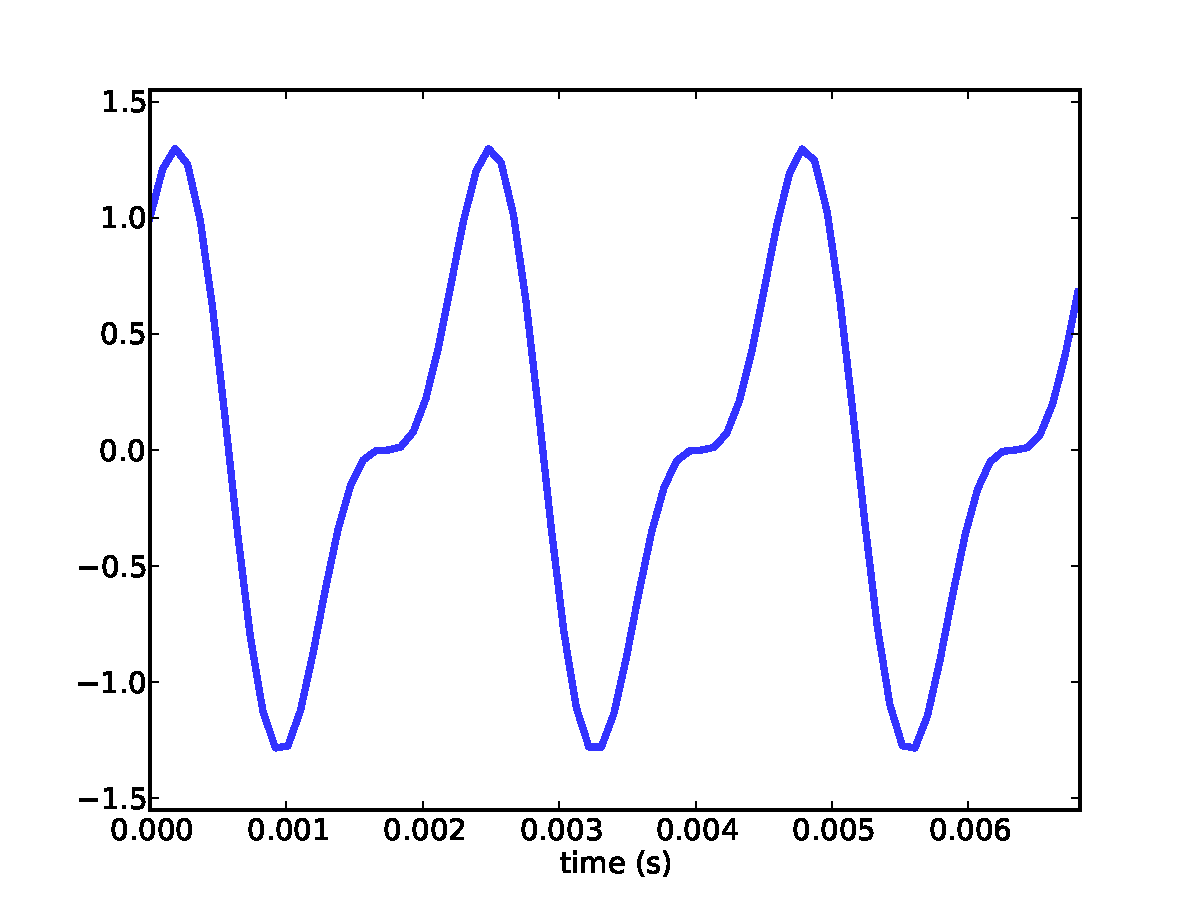
\includegraphics[height=2.5in]{figs/example1.pdf}}
\caption{Segment from a mixture of two sinusoid signals.}
\label{fig.example1}
\end{figure}

At {\tt freq=440} there are 220 periods in 0.5 seconds, so this plot
would look like a solid block of color.  To zoom in on a small number
of periods, we can use {\tt segment}, which copies a segment of a Wave
and returns a new wave:

\begin{verbatim}
    period = mix.period
    segment = wave.segment(start=0, duration=period*3)
\end{verbatim}

{\tt period} is a property of a Signal; it returns the period in second.

{\tt start} and {\tt duration} are in seconds.  This example copies
the first three periods from {\tt mix}.  If we plot {\tt segment}, it
looks like Figure~\ref{fig.example1}.  This signal contains two
frequency components, so it is more complex than the signal from the
tuning fork, but less complex than the violin.


\section{Reading and writing Waves}

{\tt thinkdsp} provides \verb"read_wave", which reads a WAV
file and returns a Wave:

\begin{verbatim}
    violin_wave = thinkdsp.read_wave('violin1.wav')
\end{verbatim}

And {\tt Wave} provides {\tt write}, which writes a WAV file:

\begin{verbatim}
    wave.write(filename='example1.wav')
\end{verbatim}

You can listen to the Wave with any media player that plays WAV
files.  On UNIX systems, I use {\tt aplay}, which is simple, robust,
and included in many Linux distributions.  For Windows you might like
MicroWav, available from
\url{http://bellsouthpwp2.net/b/o/bobad/microwav.htm}.

{\tt thinkdsp} also provides \verb"play_wave", which runs
the media player as a subprocess:

\begin{verbatim}
    thinkdsp.play_wave(filename='example1.wav', player='aplay')
\end{verbatim}

It uses {\tt aplay} by default, but you can provide another player.


\section{Spectrums}

{\tt Wave} provides \verb"make_spectrum", which returns a
{\tt Spectrum}:

\begin{verbatim}
    spectrum = wave.make_spectrum()
\end{verbatim}

And {\tt Spectrum} provides {\tt plot}:

\begin{verbatim}
    spectrum.plot()
    thinkplot.show()
\end{verbatim}

{\tt thinkplot} is a module I wrote to provide wrappers around some of
the functions in {\tt pyplot}.  You can download it from
\url{http://think-dsp.com/thinkplot.py}.  It is also included in the
Git repository for this book (see Section~\ref{code}).

{\tt Spectrum} provides three methods that modify the spectrum:

\begin{itemize}

\item \verb"low_pass" applies a low-pass filter, which means that
  components above a given cutoff frequency are attenuated (that is,
  reduced in magnitude) by a factor.

\item \verb"high_pass" applies a high-pass filter, which means that
  it attenuates components below the cutoff.

\item \verb"band_stop" attenuates components in a the band of
frequencies between two cutoffs.

\end{itemize}

This example attenuates all frequencies above 600 by 99\%:

\begin{verbatim}
   spectrum.low_pass(cutoff=600, factor=0.01)
\end{verbatim}

Finally, you can convert a Spectrum back to a Wave:

\begin{verbatim}
    wave = spectrum.make_wave()
\end{verbatim}

At this point you know how to use many of the classes and functions in
{\tt thinkdsp}, and you are ready to do the exercises at the end of
the chapter.  In Chapter~\ref{harmonics} I explain more
about how these classes are implemented.



\section{Exercises}

\begin{exercise}
Read the thinkdsp documentation.
\end{exercise}

\begin{exercise}
Fork and clone the repo.
\end{exercise}

\begin{exercise}
The example code in this chapter is in {\tt example1.py}.  If you
run it, it should ...

Gradually increase the cutoff and listen...
\end{exercise}

\begin{exercise}
Run violin.py and listen.
\end{exercise}

\begin{exercise}
Create exercise1.py and copy example1.py

Record a WAV file, or download from ...

Use an audio editor to examine the wave

Find a section where the wave is periodic and plot a few periods.

Compute and plot the spectrum.
\end{exercise}

\begin{exercise}
Extract a 0.5-2 second segment with constant frequency.

Compute the spectrum.

Remove some of the harmonics, invert the transform and play the wave.
\end{exercise}

\begin{exercise}
Synthesize a wave by creating a spectrum with arbitrary harmonics,
inverting it, and listening.  What happens as you add frequency
components that are not multiples of the fundamental?
\end{exercise}

\begin{exercise}
This exercise asks you to write a function that simulates the
effect of sound transmission underwater.
This is a more open-ended exercise for ambitious readers.
It uses decibels, which you can read about at
\url{http://en.wikipedia.org/wiki/Decibel}.

First some background information: when sound travels through water,
high frequency components are absorbed more than low frequency
components.  In pure water, the absorption rate, expressed in decibels
per kilometer (dB/km), is proportional to frequency squared.

For example, if the absorption rate for frequency $f$ is 1 dB/km,
we expect the absorption rate for $2f$ to be 4 dB/km.  In other words,
doubling the frequency quadruples the absorption rate.

Over a distance of 10 kilometers, the $f$ component would be attenuated
by 10 dB, which corresponds to a factor of 10 in power, or a factor
of 3.162 in amplitude.  

Over the same distance, the $2f$ component would be attenuated by
40 dB, or a factor or 100 in amplitude.

Write a function that takes a Wave and returns a new Wave that contains
the same frequency components as the original, but where each
component is attenuated according to the absorption rate of water.
Apply this function to the violin recording to see what a violin
would sound like under water.

For more about the physics of sound transmission in water, see
``Underlying physics and mechanisms for the absorption of sound in
seawater'' at
\url{http://resource.npl.co.uk/acoustics/techguides/seaabsorption/physics.html}

\end{exercise}




\chapter{Harmonics}
\label{harmonics}


\section{Implementing Signals and Spectrums}

If you have done the exercises, you know how to use the classes and
methods in {\tt thinkdsp}.  Now let's see how they work.

We'll start with {\tt CosSignal} and {SinSignal}:

\begin{verbatim}
def CosSignal(freq=440, amp=1.0, offset=0):
    return Sinusoid(freq, amp, offset, func=numpy.cos)

def SinSignal(freq=440, amp=1.0, offset=0):
    return Sinusoid(freq, amp, offset, func=numpy.sin)
\end{verbatim}

These functions are just wrappers for {\tt Sinusoid}, which
is a kind of Signal:

\begin{verbatim}
class Sinusoid(Signal):
    
    def __init__(self, freq=440, amp=1.0, offset=0, func=numpy.sin):
        Signal.__init__(self)
        self.freq = freq
        self.amp = amp
        self.offset = offset
        self.func = func
\end{verbatim}

The parameters of \verb"__init__" are:

\begin{itemize}

\item {\tt freq}: frequency in cycles per second, or Hz.

\item {\tt amp}: amplitude.  The units of amplitude are arbitrary,
usually chosen so 1.0 corresponds to the maximum input from a
microphone or maximum output to a speaker.

\item {\tt offset}: where in its period the signal starts, at $t=0$.
In units of radians, for reasons I explain below.

\item {\tt func}: a Python function used
to evaluate the signal at a particular point in time.  It is
usually either {\tt numpy.sin} or {\tt numpy.cos}, yielding a sine or
cosine signal.

\end{itemize}

Like many \verb"__init__" methods, this one just tucks the
parameters away for future use.

The parent class of {\tt Sinusoid}, {\tt Signal}, provides \verb"make_wave":

\begin{verbatim}
    def make_wave(self, duration=1, start=0, framerate=11025):
        dt = 1.0 / framerate
        ts = numpy.arange(start, duration, dt)
        ys = self.evaluate(ts)
        return Wave(ys, framerate)
\end{verbatim}

{\tt start} and {\tt duration} are the start time and duration
in seconds.  {\tt framerate} is the number of frames (samples)
per second.

{\tt dt} is the time between samples, and {\tt ts} is the sequence
of sample times.

\verb"make_wave" invokes {\tt evaluate}, which has to be provided
by the child class of {\tt Signal}, in this case {\tt Sinusoid}.

{\tt evaluate} takes the sequence of samples times and returns an array of
corresponding quantities:

\begin{verbatim}
    def evaluate(self, ts):
        phases = PI2 * self.freq * ts + self.offset
        ys = self.amp * self.func(phases)
        return ys
\end{verbatim}

{\tt ts} and {\tt ys} are NumPy arrays.  I use NumPy and SciPy
throughout the book.  If you are familiar with these libraries,
that's great, but I will also explain as we go along.

Let's unwind this function one step at time:

\begin{enumerate}

\item {\tt self.freq} is frequency in cycles per second, and
each element of {\tt ts} a time in seconds, so their product is
the number of cycles since the start time.

\item {\tt PI2} is a constant that stores $2 \pi$.  Multiplying
by {\tt PI2} converts from cycles to {\bf phase}.  You can
think of phase as ``cycles since the start time'' except that the number
of cycles is in units of radians, so each cycle is $2 \pi$ radians.

\item {\tt self.offset} is the phase, in radians, at the start time.
  It has the effect of shifting the signal left or right in time.

\item If {\tt self.func} is {\tt sin} or {\tt cos}, the result is a
  value between $-1$ and $+1$.

\item Multiplying by {\tt self.amp} yields a signal that ranges from
  {\tt -self.amp} to {\tt +self.amp}.

\end{enumerate}

In math notation, {\tt evaluate} is written like this:

\[ A \cos (2 \pi f t + \phi) \]

where $A$ is amplitude, $f$ is frequency, $t$ is time, and $\phi$
is the phase offset.  It may seem like I wrote a lot of code
to evaluate one simple function, but as we will see, this code
provides a framework for dealing with all kinds of signals, not
just sinusoids.


\section{Computing the spectrum}

Given a Signal, we can compute a Wave.  Given a Wave, we can compute
a Spectrum.  {\tt Wave} provides \verb"make_spectrum", which returns
a new {\tt Spectrum} object.

\begin{verbatim}
    def make_spectrum(self):
        hs = numpy.fft.rfft(self.ys)
        return Spectrum(hs, self.framerate)
\end{verbatim}

\verb"make_spectrum" uses {\tt rfft}, which computes
the discrete Fourier transform using an algorithm called
{\bf Fast Fourier Transform} or FFT.

The result of {\tt fft} is a sequence of complex numbers, {\tt hs},
which is stored in a Spectrum.  There are two ways to think about
complex numbers:

\begin{itemize}

\item A complex number is the sum of a real part and an imaginary
part, often written $x + iy$, where $i$ is the imaginary unit, $\sqrt{-1}$.
You can think of $x$ and $y$ as Cartesian coordinates.

\item A complex number is also the product of a magnitude
and a complex exponential, $r e^{i \phi}$, where $r$ is the
{\bf magnitude} and $\phi$ is the
{\bf angle} in radians, also called the ``argument.''   You
can think of $r$ and $\phi$ as polar coordinates.

\end{itemize}

Each element of {\tt hs} corresponds to a
frequency component.  The magnitude of each element is proportional
to the amplitude of the corresponding component.
The angle of each element is the phase offset (relative to a cosine
signal).

{\tt NumPy} provides {\tt absolute}, which computes
the magnitude of a complex number, also called the ``absolute value,''
and {\tt angle}, which computes the angle.

Here is the definition of {\tt Spectrum}:

\begin{verbatim}
class Spectrum(object):

    def __init__(self, hs, framerate):
        self.hs = hs
        self.framerate = framerate

        n = len(hs)
        f_max = framerate / 2.0
        self.fs = numpy.linspace(0, f_max, n)

        self.amps = numpy.absolute(self.hs)
\end{verbatim}

Again, {\tt hs} is the result of the FFT and {\tt framerate}
is the number of frames per second.

The elements of {\tt hs} correspond to a sequence of frequencies, {\tt
  fs}, equally spaced from 0 to the maximum frequency, \verb"f_max".
The maximum frequency is {\tt framerate/2}, for reasons we'll see
soon.

Finally, {\tt amps} contains the magnitude of {\tt hs}, which
is proportional to the amplitude of the components.

{\tt Spectrum} also provides {\tt plot}, which plots the magnitude for each
frequency:

\begin{verbatim}
    def plot(self, low=0, high=None):
        thinkplot.Plot(self.fs[low:high], self.amps[low:high])
\end{verbatim}

{\tt low} and {\tt high} specify the slice of the Spectrum that
should be plotted.


\section{Other waveforms}

A sinusoid contains only one frequency component, so its DFT
has only one peak.  More complex waveforms, like the
violin recording, yield DFTs with many peaks.  In this section we
investigate the relationship between waveforms and their DFTs.

\begin{figure}
% example2.py
\centerline{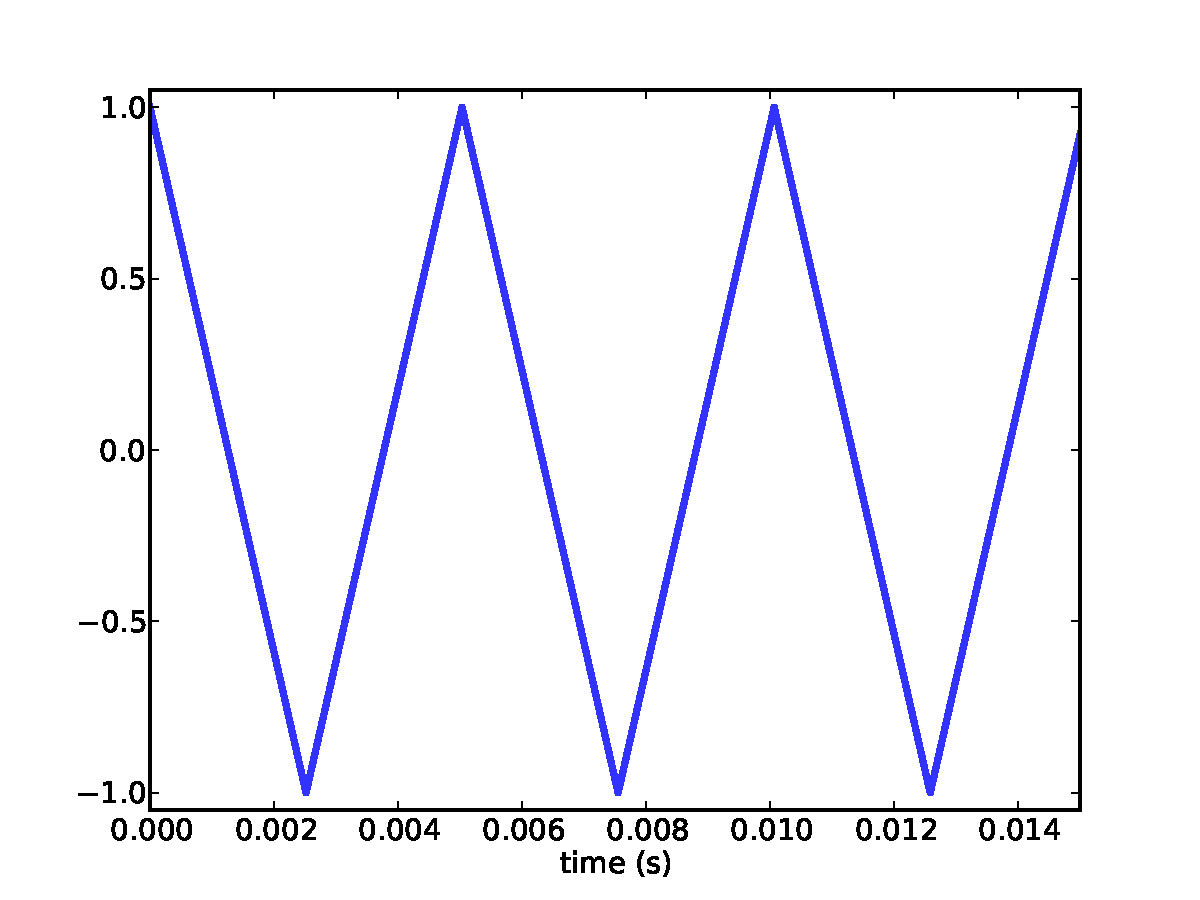
\includegraphics[height=2.5in]{figs/triangle-200-1.pdf}}
\caption{Segment of a triangle signal at 200 Hz.}
\label{fig.triangle.200.1}
\end{figure}

The triangle waveform is like a straight-line version of a sinusoid.
Figure~\ref{fig.triangle.200.1} shows a triangle waveform with
frequency 200 Hz.

To generate a triangle wave, you can use {\tt thinkdsp.TriangleSignal}:

\begin{verbatim}
class TriangleSignal(Sinusoid):
    
    def evaluate(self, ts):
        cycles = self.freq * ts + self.offset / PI2
        frac, _ = numpy.modf(cycles)
        ys = numpy.abs(frac - 0.5)
        ys = normalize(unbias(ys), self.amp)
        return ys
\end{verbatim}

{\tt TriangleSignal} inherits \verb"__init__" from {\tt Sinusoid},
so it takes the same arguments: {\tt freq}, {\tt amp}, and {\tt offset}.

The only difference is {\tt evaluate}.  As we saw before,
{\tt ts} is the sequence of sample times where we want to
evaluate the signal.

There are lots of ways to generate a triangle wave.  The details
are not important, but here's how {\tt evaluate} works:

\begin{enumerate}

\item {\tt cycles} is the number of cycles since the start time.
{\tt numpy.modf} splits the number of cycles into the fraction
part, stored in {\tt frac}, and the integer part, which is ignored.
\footnote{Using an underscore as a variable name is a convention that
means, ``I don't intend to use this value.''}

\item {\tt frac} is a sequence that ramps from 0 to 1 with the given
frequency.  Subtracting
0.5 yields values between -0.5 and 0.5.  Taking the absolute value
yields a waveform that zig-zags between 0.5 and 0.

\item {\tt unbias} shifts the waveform down so it is centered at 0, then
{\tt normalize} scales it to the given amplitude, {\tt amp}.

\end{enumerate}

Here's the code that generates Figure~\ref{fig.triangle.200.1}:

\begin{verbatim}
    signal = thinkdsp.TriangleSignal(200)
    duration = signal.period*3
    segment = signal.make_wave(duration, framerate=10000)
    segment.plot()
\end{verbatim}


\section{Harmonics}

Next we can compute the spectrum of this waveform:

\begin{verbatim}
    wave = signal.make_wave(duration=0.5, framerate=framerate)
    spectrum = wave.make_spectrum()
    spectrum.plot()
\end{verbatim}

\begin{figure}
% example2.py
\centerline{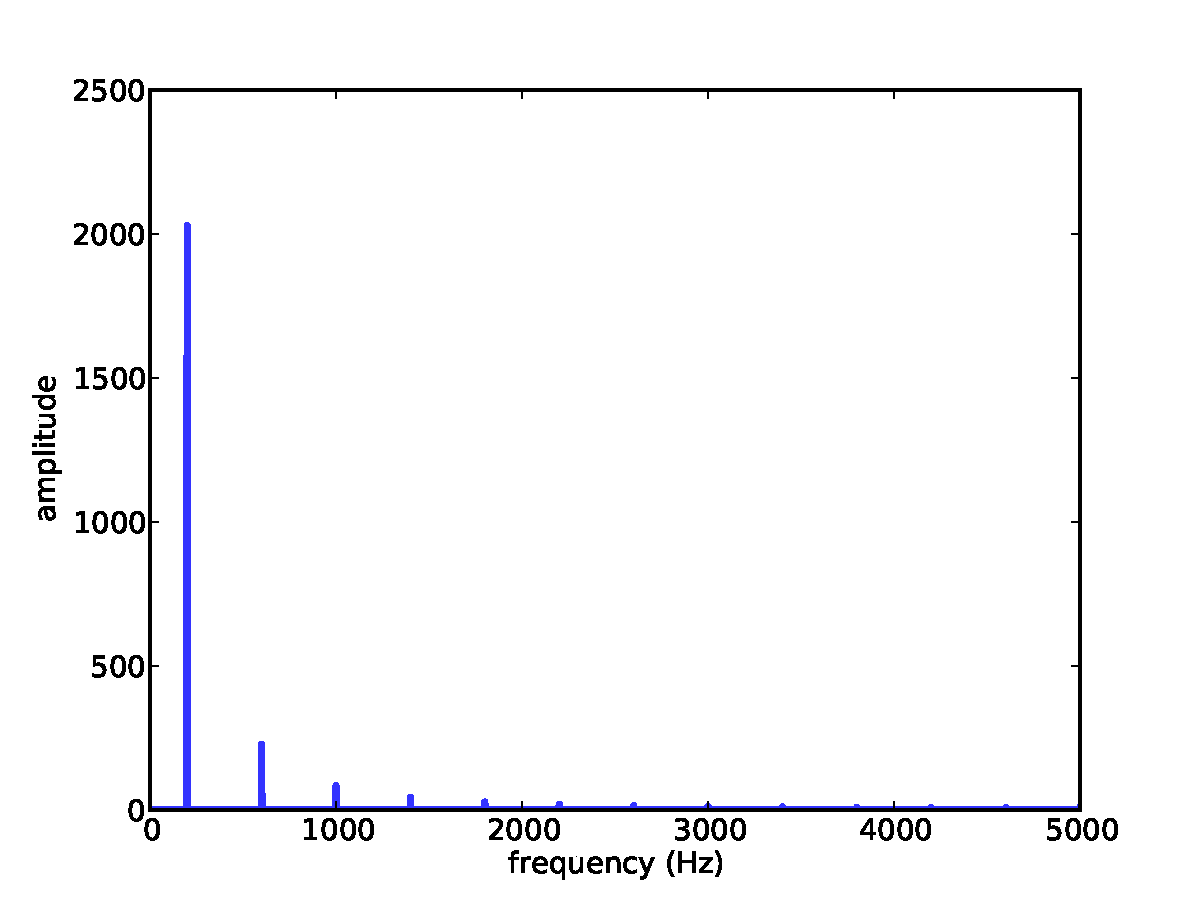
\includegraphics[height=2.5in]{figs/triangle-200-2.pdf}}
\caption{Spectrum of a triangle signal at 200 Hz.}
\label{fig.triangle.200.2}
\end{figure}

Figure~\ref{fig.triangle.200.2} shows the result.  As expected, the
highest peak is at the fundamental frequency, 200 Hz, and there
are additional peaks at harmonic frequencies, which are integer
multiples of 200.

But one surprise is that there are no peaks at the even multiples:
400, 800, etc.  The harmonics of a triangle wave are all
odd multiples of the fundamental frequency, in this example
600, 1000, 1400, etc.

Another feature of this spectrum is the relationship between the
amplitude and frequency of the harmonics.  The amplitude of the
harmonics drops off in proportion to frequency squared.  For example
the frequency ratio of the first two harmonics (200 and 600 Hz) is 3, and the
amplitude ration is approximately 9.  The frequency ratio of the
next two harmonics (600 and 1000 Hz) is 1.7, and the amplitude ratio
is approximately $1.7^2 = 2.9$.

{\tt thinkdsp} also provides {\tt SquareSignal}, which represents
a square signal.  Here's the class definition:

\begin{verbatim}
class SquareSignal(Sinusoid):
    
    def evaluate(self, ts):
        cycles = self.freq * ts + self.offset / PI2
        frac, _ = numpy.modf(cycles)
        ys = self.amp * numpy.sign(unbias(frac))
        return ys
\end{verbatim}

Like {\tt TriangleSignal}, {\tt SquareSignal} inherits 
\verb"__init__" from {\tt Sinusoid}, so it takes the same
parameters.

And the {\tt evaluate} method is similar.  Again, {\tt cycles} is
the number of cycles since the start time, and {\tt frac} is the
fractional part, which ramps from 0 to 1 each period.

{\tt unbias} shifts {\tt frac} so it ramps from -0.5 to 0.5,
then {\tt numpy.sign} maps the negative values to -1 and the
positive values to 1.  Multiplying by {\tt amp} yields a square
wave that jumps between {\tt -amp} and {\tt amp}.

\begin{figure}
% example2.py
\centerline{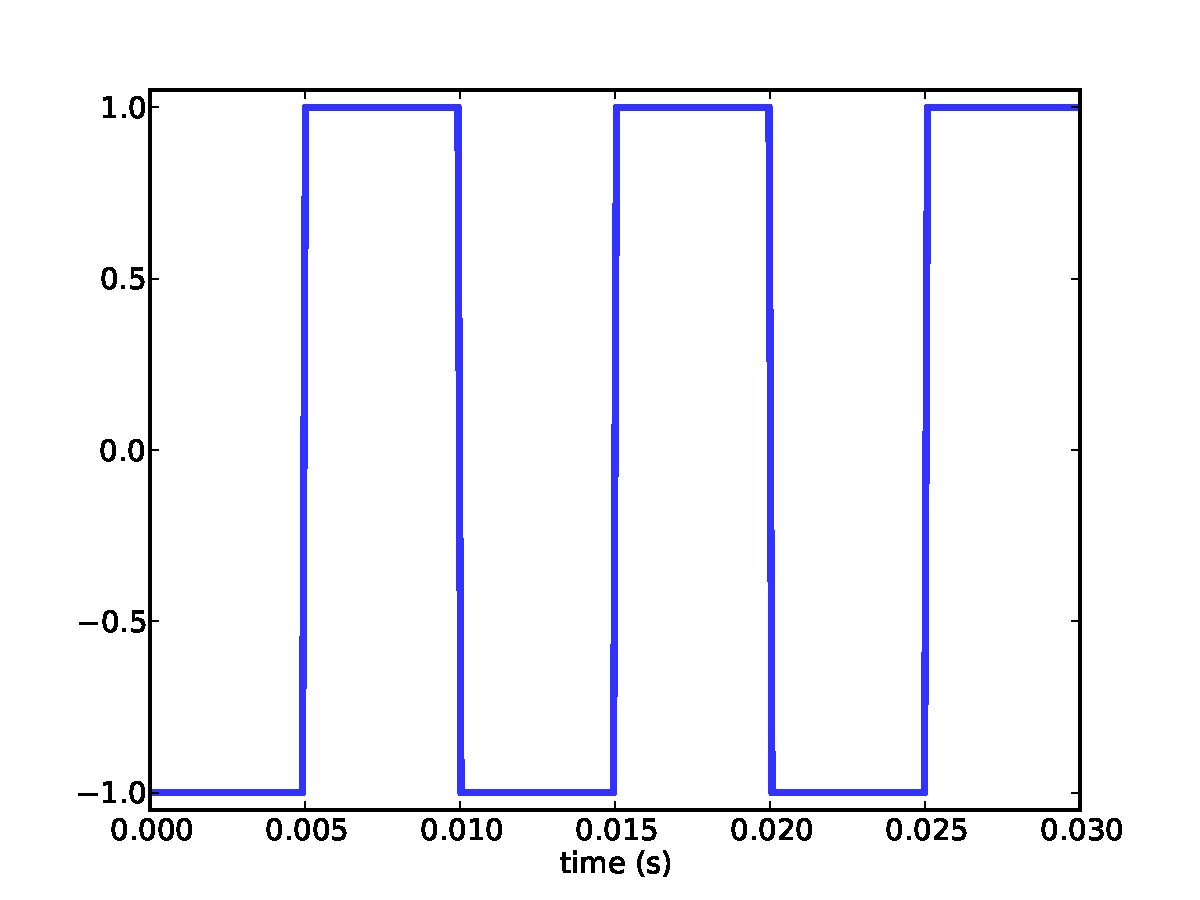
\includegraphics[height=2.5in]{figs/square-100-1.pdf}}
\caption{Segment of a square signal at 100 Hz.}
\label{fig.square.100.1}
\end{figure}

\begin{figure}
% example2.py
\centerline{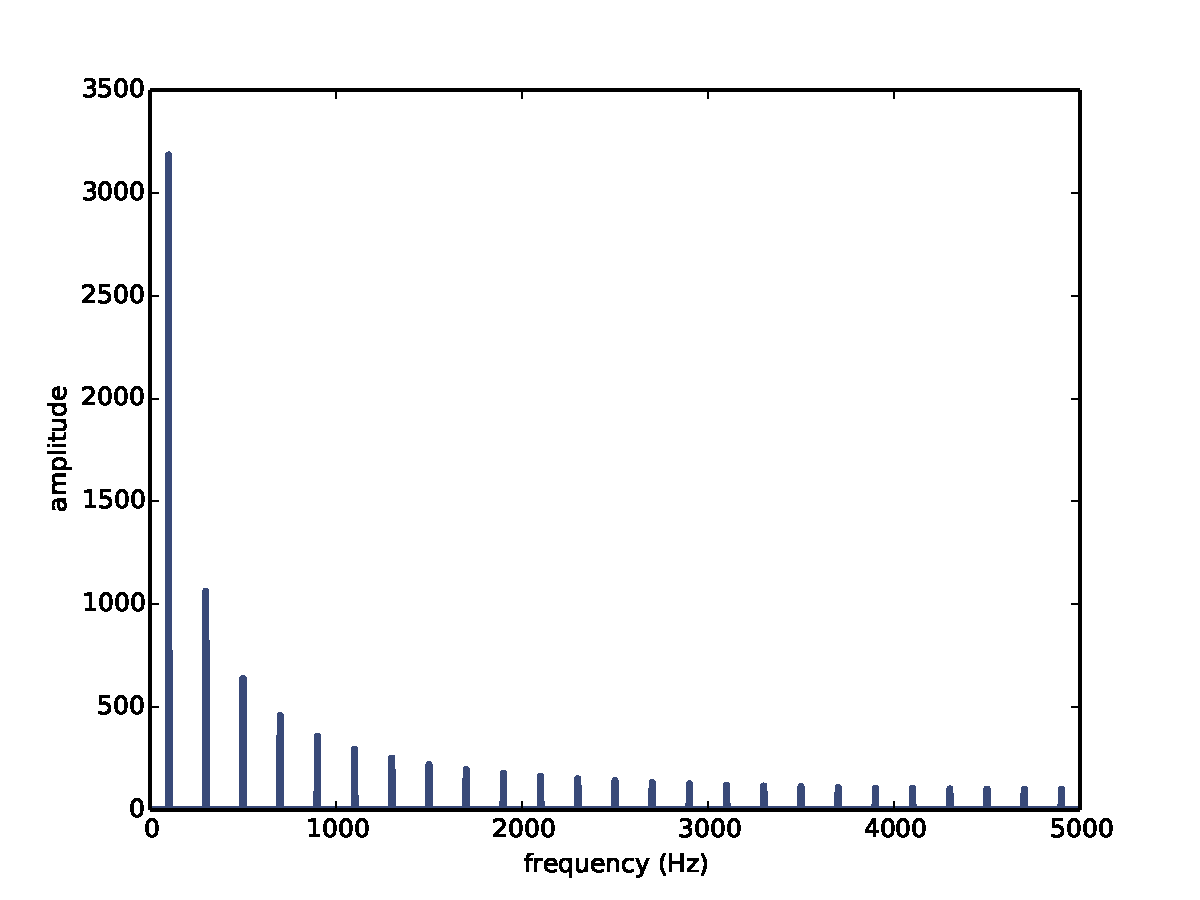
\includegraphics[height=2.5in]{figs/square-100-2.pdf}}
\caption{Spectrum of a square signal at 100 Hz.}
\label{fig.square.100.2}
\end{figure}

Figure~\ref{fig.square.100.1} shows three periods of a square
wave with frequency 100 Hz,
and Figure~\ref{fig.square.100.2} shows its spectrum.

Like a triangle wave, the square wave contains only odd harmonics,
which is why there are peaks at 300, 500, and 700 Hz, etc.
But the amplitude of the harmonics drops off more slowly.
Specifically, amplitude drops in proportion to frequency (not frequency
squared).


\section{Aliasing}

\begin{figure}
% example2.py
\centerline{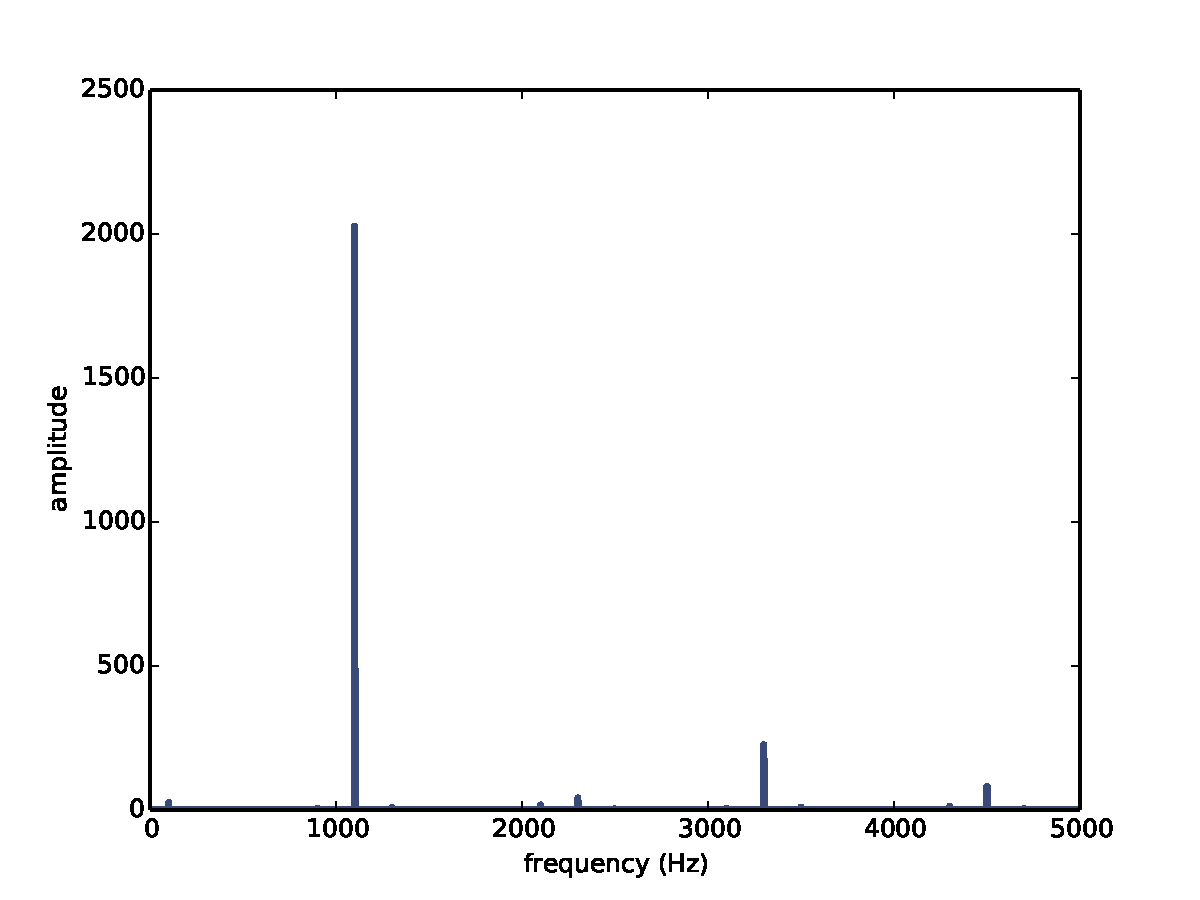
\includegraphics[height=2.5in]{figs/triangle-1100-2.pdf}}
\caption{Spectrum of a triangle signal at 1100 Hz sampled at
10,000 frames per second.}
\label{fig.triangle.1100.2}
\end{figure}

I have a confession.  I chose the examples in the previous section
carefully,
to avoid showing you something confusing.  But now it's time to get
confused.

Figure~\ref{fig.triangle.1100.2} shows the spectrum of a triangle wave at 1100 Hz, sampled
at 10,000 frames per second.

As expected, there are peaks at 1100 and 3300 Hz, but the third
peak is at 4500, not 5500 Hz as expected.  There is a small fourth peak
at 2300, not 7700 Hz.  And if you look very closely, the peak that should
be at 9900 is actually at 100 Hz.  What's going on?

The fundamental problem is that when you evaluate the signal at
discrete points in time, you lose information about what happens
between samples.  For low frequency components, that's not a
problem, because you have lots of samples per period.

But if you sample a signal at 5000 Hz with 10,000 frames per second,
you only have two samples per period.  That's enough to measure the
frequency (it turns out), but it doesn't tell you much about
the shape of the signal.

If the frequency is higher, like the 5500 Hz component of the
triangle wave, things are worse: you don't even get the
frequency right.

To see why, let's generate cosine signals at 4500 and 5500 Hz,
and sample them at 10,000 frames per second:

\begin{verbatim}
    framerate = 10000

    signal = thinkdsp.CosSignal(4500)
    duration = signal.period*5
    segment = signal.make_wave(duration, framerate=framerate)
    segment.plot()

    signal = thinkdsp.CosSignal(5500)
    segment = signal.make_wave(duration, framerate=framerate)
    segment.plot()
\end{verbatim}

\begin{figure}
% example2.py
\centerline{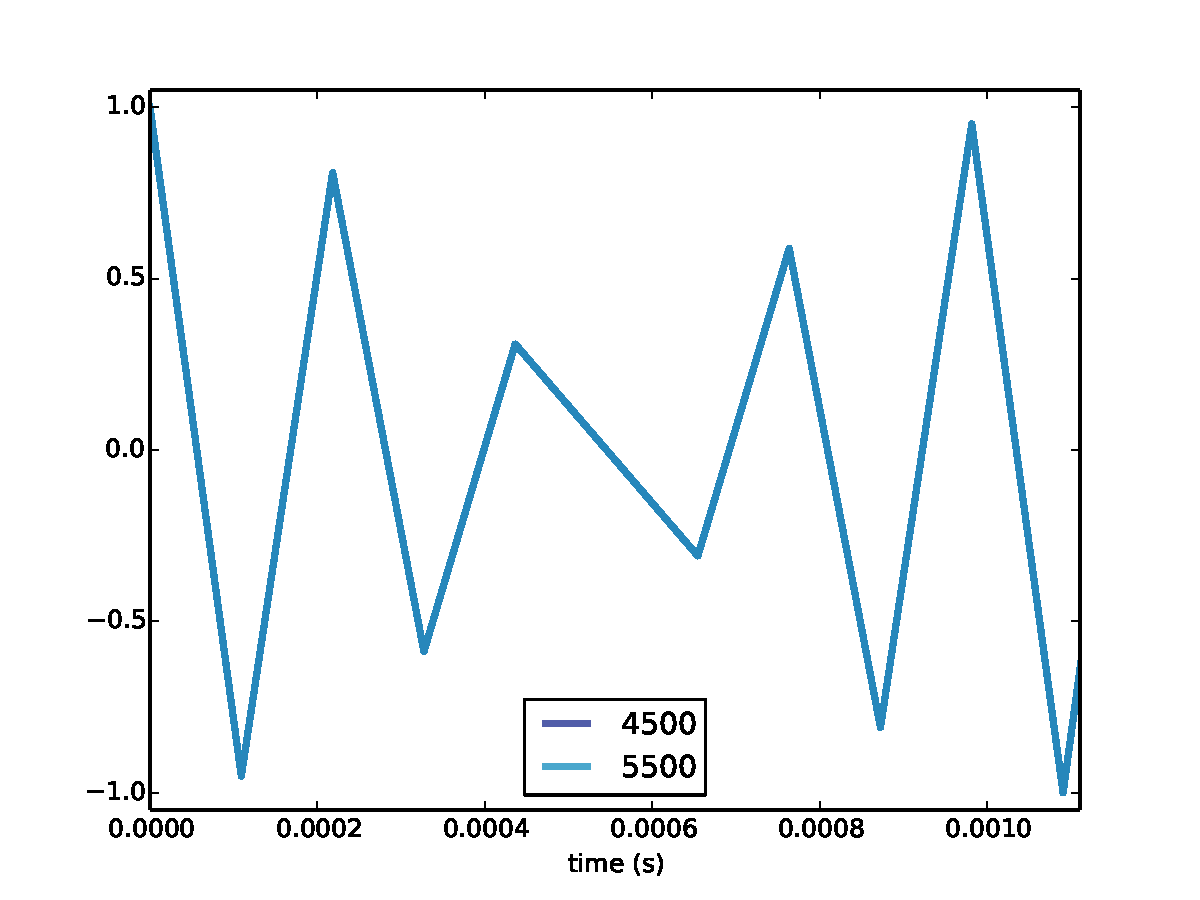
\includegraphics[height=2.5in]{figs/aliasing-3.pdf}}
\caption{Cosine signals at 4500 and 5500 Hz, sampled at 10,000 frames
per second.}
\label{fig.aliasing-3}
\end{figure}

Figure~\ref{fig.aliasing-3} shows the result.  The
sampled waveform doesn't look very much like a sinusoid, but the
bigger problem is that the two waveforms are exactly the same!

When we sample a 5500 Hz signal at 10,000 frames per second, the
result is indistinguishable from a 4500 Hz signal.

For the same reason, a 7700 Hz signal is indistinguishable
from 2300 Hz, and a 9900 Hz is indistinguishable from 100 Hz.

This effect is called {\bf aliasing} because when the high frequency
signal is sampled, it disguises itself as a low frequency signal.

In this example, the highest frequency we can measure is 5000 Hz,
which is half the sampling rate.  Frequencies above 5000 Hz are folded
back below 5000 Hz, which is why this threshold is sometimes called
the ``folding frequency,'' but more often it is called the {\bf
  Nyquist frequency}.  See
\url{http://en.wikipedia.org/wiki/Nyquist_frequency}.

The folding pattern continues if the aliased frequency goes below
zero.  For example, the 5th harmonic of the 1100 Hz triangle wave is
at 12,100 Hz.  Folded at 5000 Hz, it would appear at -2100 Hz, but it
gets folded again at 0 Hz, back to 2100 Hz.  In fact, you can see a
small peak at 2100 Hz in Figure~\ref{fig.square.100.2}, and the next
one at 4300 Hz.


\section{Exercises}

\begin{exercise}
Listen to the various non-sinusoidal waveforms.
\end{exercise}

\begin{exercise}
Start with a sawtooth.  Compute the DFT.  Remove all harmonics above
the $i$th.
Compute the inverse DFT and see what it looks like.
Repeat for a range of values of $i$.
\end{exercise}

\begin{exercise}
Write a new Signal type, compute it's DFT and listen to it.  What
happens if the signal is discontinuous?  What if the signal is continuous
but the slope is discontinuous?
\end{exercise}

\begin{exercise}
Make a frequency-limited sawtooth wave and see what it looks like
and sounds like.
See \url{http://en.wikipedia.org/wiki/Sawtooth_wave}.

\begin{exercise}
What does a square wave sound like underwater?
\end{exercise}

\begin{exercise}
Sample an 1100 Hz triangle at 10000 frames per second and listen to it.
Can you hear the aliased harmonic?  Might help to play a sequence of
notes with increasing pitch.
\end{exercise}

\begin{exercise}
Compute the spectrum of an 1100 Hz square wave.
\end{exercise}


\end{exercise}

\chapter{Discrete Cosine Transform}

At this point we know how to use an FFT to identify the frequency
components of a complex signal, but we don't know how it works.

To explain, I will proceed in a few steps.  Here's the outline:

\begin{enumerate}

\item We'll start with covariance, which is a measure of how similar
two signals are.

\item Then I'll present the discrete cosine transform (DFT), which compares
a signal to cosine signals with a range of frequencies.  Although the
DFT is useful for some applications, it is not sufficient for spectral
analysis because it only captures part of the signal, the so-called
``even'' part.

\item Then we'll see that the sine transform captures the other part
of the signal, the ``odd'' part.

\item We'll combine the sine and cosine transforms to make
the discrete Fourier transform (DFT).

\item And finally we'll derive the FFT, which is an efficient
  algorithm to evaluate the DFT.

\end{enumerate}

So let's get started.


\section{Covariance}

Suppose I give you a Wave that represents samples from a cosine
signal, but I don't tell you the frequency of the signal.  How would
you figure it out.

One possibility is to plot the waveform, identify the repeating
pattern, and measure the period.  From the period, you can compute
the frequency.

That would work with a simple signal, where the repeating pattern
is obvious, but it would not be easy with a complex signal containing
many frequency components.  And if the samples come from a real-world
signal, they might be noisy, which would make it even harder.

A more robust approach is to compare the given Wave to cosine
signals with a known frequencies, and see which 



generate cosine signals with a range
of frequencies, and se

\begin{verbatim}
\end{verbatim}


\begin{verbatim}
\end{verbatim}


\begin{verbatim}
\end{verbatim}


\begin{verbatim}
\end{verbatim}


\begin{verbatim}
\end{verbatim}


\begin{verbatim}
\end{verbatim}


\begin{verbatim}
\end{verbatim}


\begin{verbatim}
\end{verbatim}


\begin{verbatim}
\end{verbatim}


\begin{verbatim}
\end{verbatim}


\begin{verbatim}
\end{verbatim}


\begin{verbatim}
\end{verbatim}


\begin{verbatim}
\end{verbatim}


\begin{verbatim}
\end{verbatim}


\begin{verbatim}
\end{verbatim}


\chapter{Notes}

Case study ideas:

\begin{itemize}

\item Pitch tracking in Rock Band

\item Auto-Tune

\item JPEG compression

\item Image recognition in Fourier space (money)

\item Application of cepstrum?

\item Application of z transform -- digital control systems

\end{itemize}

\end{document}
